\documentclass[a4paper, 12pt]{article} 
\usepackage[top=2cm, bottom=2cm, left=2.5cm, right=2.5cm]{geometry}
\usepackage[utf8]{inputenc}
\usepackage{amsmath, amsfonts, amssymb}
\usepackage{graphicx} %pacote para inserir figuras
\usepackage{float} %força posicionamento da figura - para usar: subtituir [htb] por[H]
\usepackage[brazil]{babel} %força latex a escrever figura e não figure
\usepackage{indentfirst} %identa o primeiro parágrafo após uma seção
\usepackage{lipsum}

\title{ \textbf{Título do trabalho}}
\author{Maurício Barbosa da Rocha \\ mauricio.mbr@gmail.com}
\date{2020}

\begin{document}

 \maketitle  %comando para escrever o título, pular página: \newpage

 \newpage	

 \tableofcontents \newpage %insere sumário
 
 \listoffigures \newpage %insere lista de figuras 
 
 \listoftables \newpage %insere lista de tabelas
 
%------------------------------------------------------------------- INTRODUÇÃO

 \section{Introdução}
  \lipsum[10] \lipsum[10]
  
 \begin{figure}[htb]
   \centering
   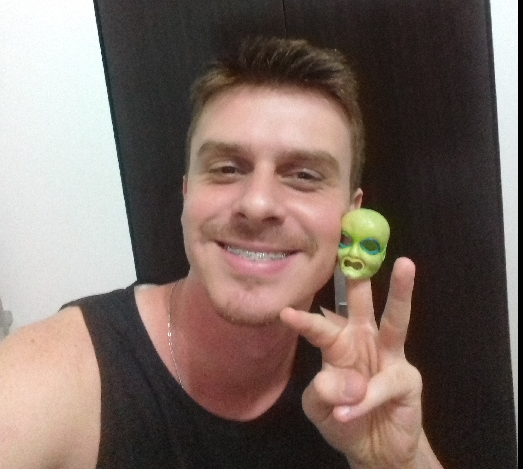
\includegraphics[scale=0.3]{imagens/eu1.png}
   \caption{Maurício e o et}
   \label{rotulo-figura1}
 \end{figure}

%------------------------------------------------------------------- DESENVOLVIMENTO  
 \section{Desenvolvimento}
  \lipsum[10]
  
 \subsection{Parte I do desenvolvimento}
 \lipsum[10]
  	 
 \subsubsection{Parte I - a do desenvolvimento}
 \lipsum[10]
  	   
 \begin{figure}[htb]
   \centering
   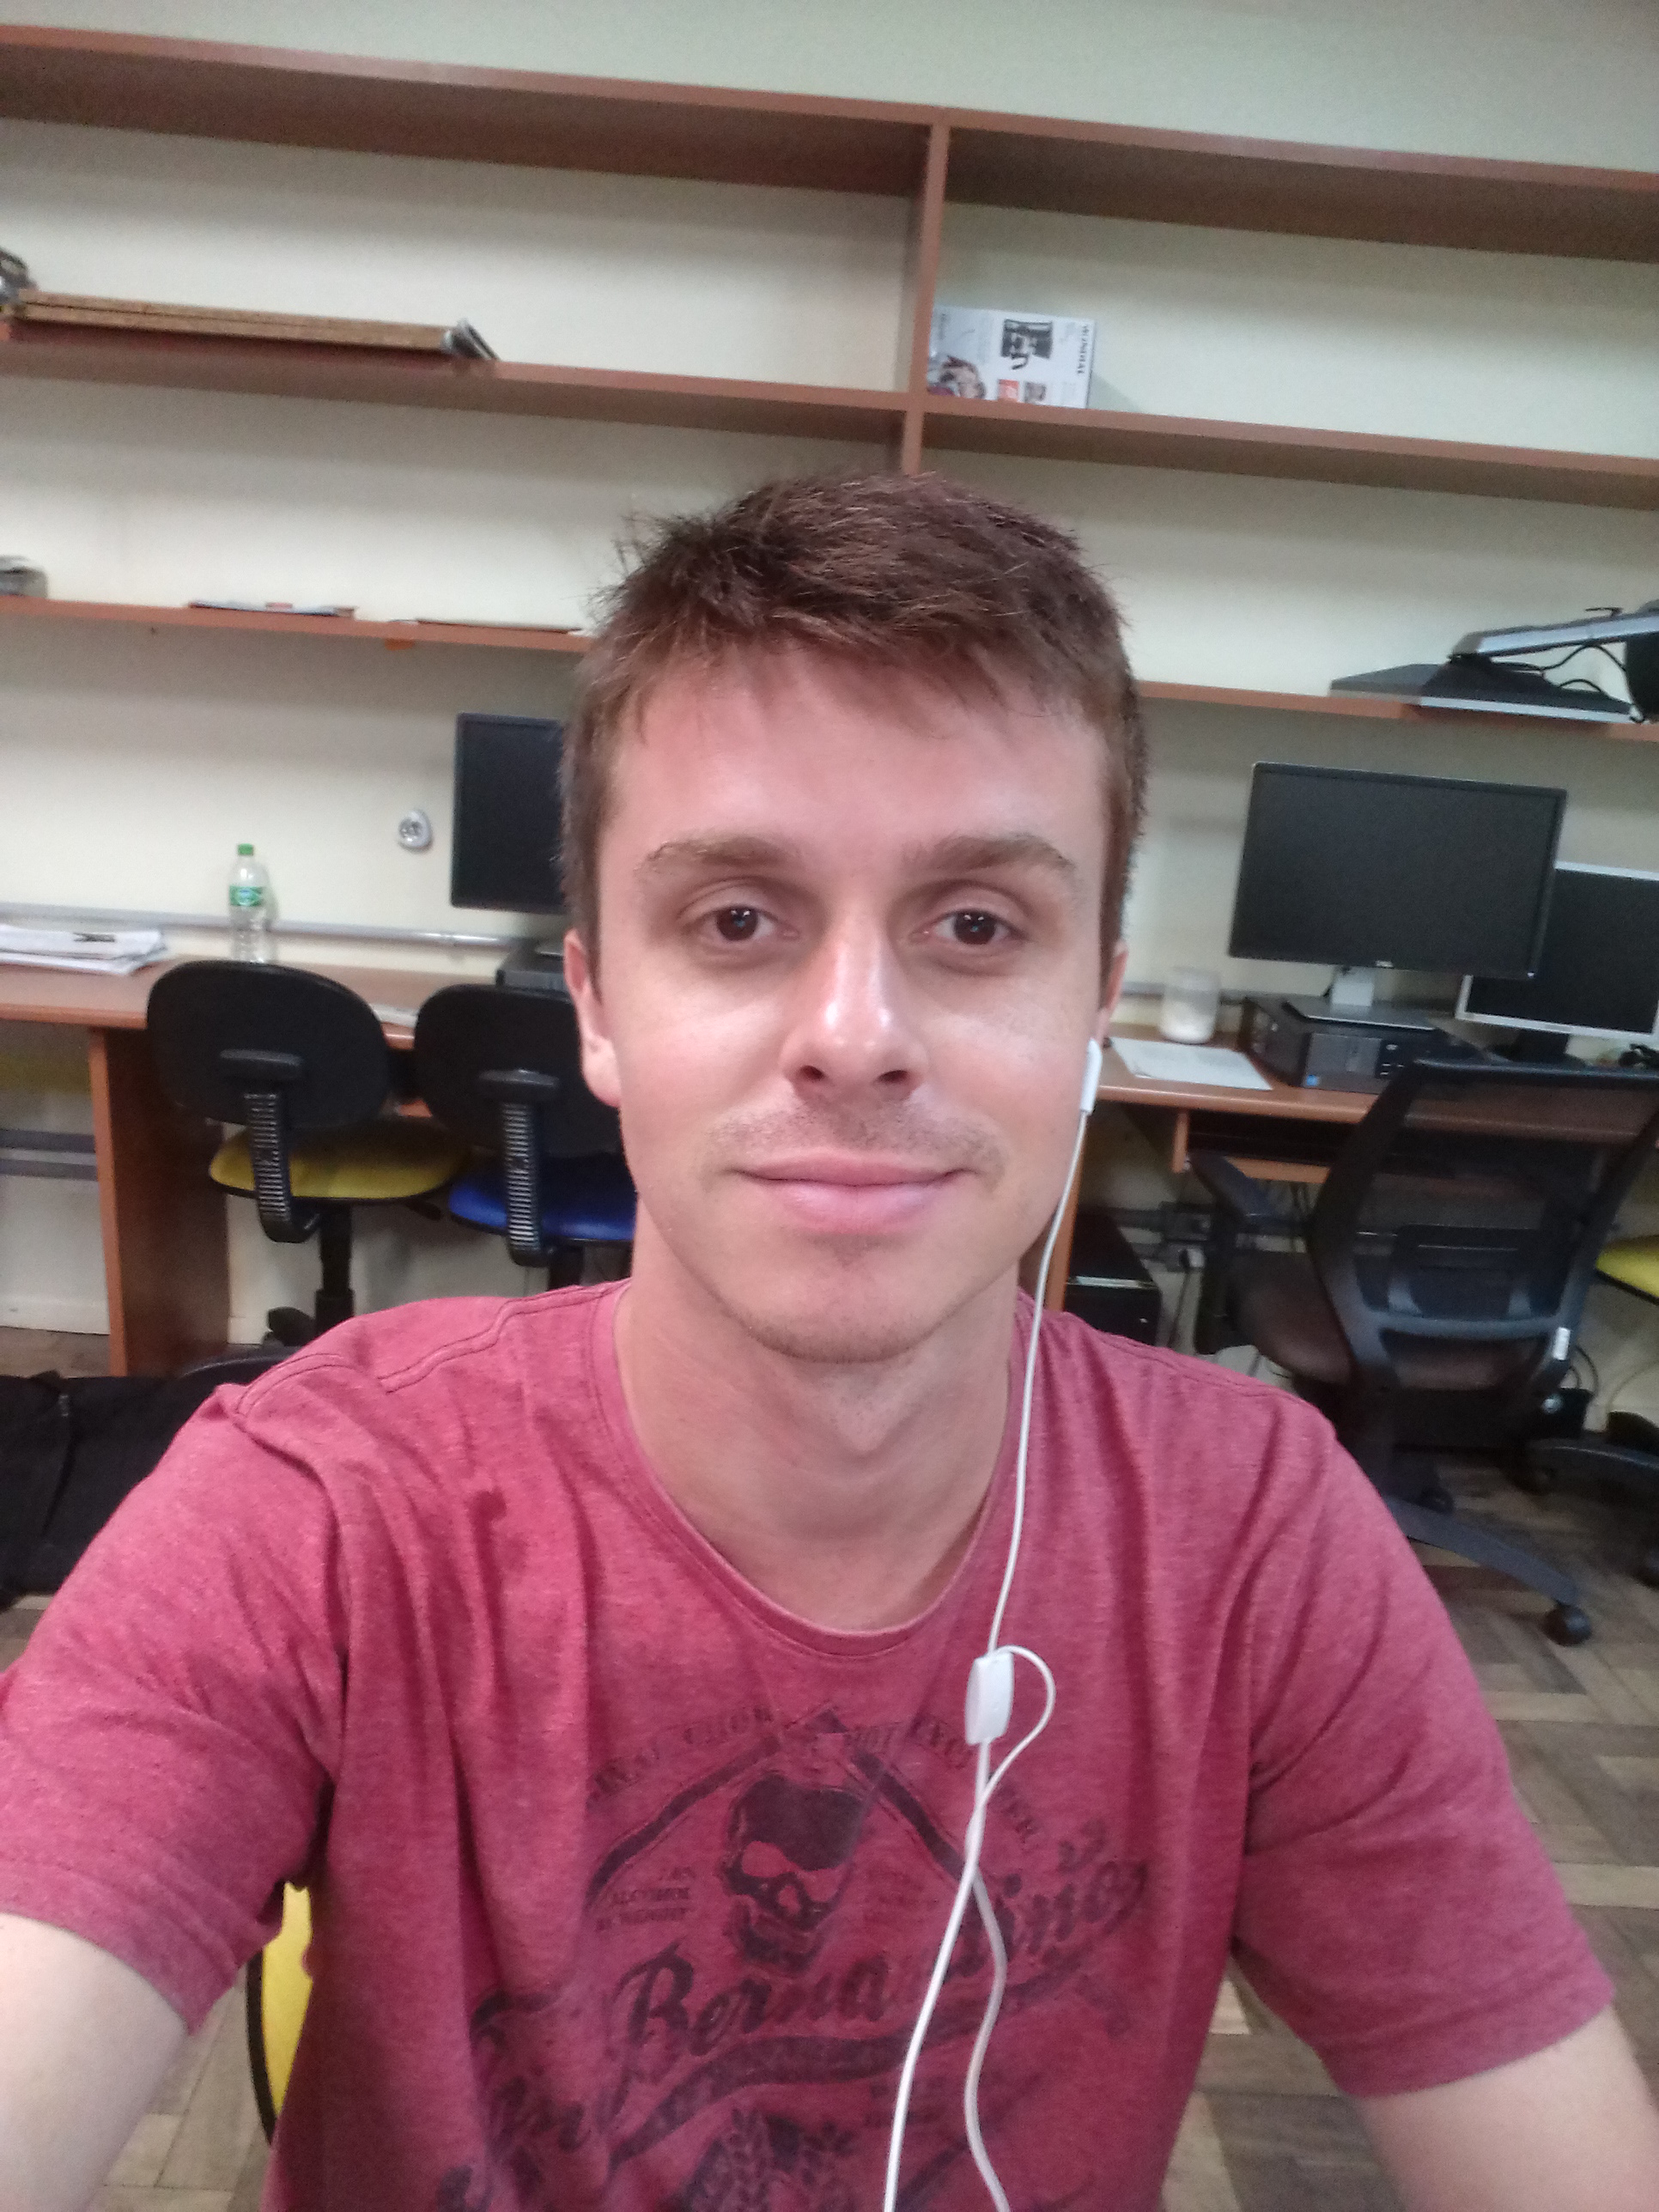
\includegraphics[scale=0.3]{imagens/eu2.jpg}
   \caption{Maurício no sensoriamento}
   \label{rotulo-figura2}
 \end{figure}
 
%------------------------------------------------------------------- CONSLUSÃO 
 \section{Conclusão}
 \lipsum[1]
 
 \begin{table}[htb]
   \centering
   \begin{tabular}{|c|c|}
     aaa1 & aaa2 \\
     aaa1 & aaa2 \\
   \end{tabular}
   \caption{Minha tabela 1}
   \label{minha-tabelinha}
 \end{table}
 
 Aqui estou citando um livro: \cite{meuatalho} 

 Aqui estou citando uma artigo: \cite{meuatalho2}
 

%------------------------------------------------------------------- REFERÊNCIAS BIBLIOGRÁFICAS
\newpage
\bibliographystyle{plain}
\addcontentsline{toc}{section}{Referências} %adiciona referencias ao sumário
\bibliography{referencia.bib} %nome do arquivo que contem as bibliografias Usar F11 para compilar

\end{document}